% Generated by Sphinx.
\def\sphinxdocclass{report}
\documentclass[letterpaper,10pt,english]{sphinxmanual}
\usepackage[utf8]{inputenc}
\DeclareUnicodeCharacter{00A0}{\nobreakspace}
\usepackage{cmap}
\usepackage[T1]{fontenc}
\usepackage{babel}
\usepackage{times}
\usepackage[Bjarne]{fncychap}
\usepackage{longtable}
\usepackage{sphinx}
\usepackage{multirow}

\addto\captionsenglish{\renewcommand{\figurename}{Fig. }}
\addto\captionsenglish{\renewcommand{\tablename}{Table }}
\floatname{literal-block}{Listing }



\title{Fingerprint Scanner Robot Documentation}
\date{July 17, 2015}
\release{1.1}
\author{Jacob Glueck}
\newcommand{\sphinxlogo}{}
\renewcommand{\releasename}{Release}
\makeindex

\makeatletter
\def\PYG@reset{\let\PYG@it=\relax \let\PYG@bf=\relax%
    \let\PYG@ul=\relax \let\PYG@tc=\relax%
    \let\PYG@bc=\relax \let\PYG@ff=\relax}
\def\PYG@tok#1{\csname PYG@tok@#1\endcsname}
\def\PYG@toks#1+{\ifx\relax#1\empty\else%
    \PYG@tok{#1}\expandafter\PYG@toks\fi}
\def\PYG@do#1{\PYG@bc{\PYG@tc{\PYG@ul{%
    \PYG@it{\PYG@bf{\PYG@ff{#1}}}}}}}
\def\PYG#1#2{\PYG@reset\PYG@toks#1+\relax+\PYG@do{#2}}

\expandafter\def\csname PYG@tok@gd\endcsname{\def\PYG@tc##1{\textcolor[rgb]{0.63,0.00,0.00}{##1}}}
\expandafter\def\csname PYG@tok@gu\endcsname{\let\PYG@bf=\textbf\def\PYG@tc##1{\textcolor[rgb]{0.50,0.00,0.50}{##1}}}
\expandafter\def\csname PYG@tok@gt\endcsname{\def\PYG@tc##1{\textcolor[rgb]{0.00,0.27,0.87}{##1}}}
\expandafter\def\csname PYG@tok@gs\endcsname{\let\PYG@bf=\textbf}
\expandafter\def\csname PYG@tok@gr\endcsname{\def\PYG@tc##1{\textcolor[rgb]{1.00,0.00,0.00}{##1}}}
\expandafter\def\csname PYG@tok@cm\endcsname{\let\PYG@it=\textit\def\PYG@tc##1{\textcolor[rgb]{0.25,0.50,0.56}{##1}}}
\expandafter\def\csname PYG@tok@vg\endcsname{\def\PYG@tc##1{\textcolor[rgb]{0.73,0.38,0.84}{##1}}}
\expandafter\def\csname PYG@tok@m\endcsname{\def\PYG@tc##1{\textcolor[rgb]{0.13,0.50,0.31}{##1}}}
\expandafter\def\csname PYG@tok@mh\endcsname{\def\PYG@tc##1{\textcolor[rgb]{0.13,0.50,0.31}{##1}}}
\expandafter\def\csname PYG@tok@cs\endcsname{\def\PYG@tc##1{\textcolor[rgb]{0.25,0.50,0.56}{##1}}\def\PYG@bc##1{\setlength{\fboxsep}{0pt}\colorbox[rgb]{1.00,0.94,0.94}{\strut ##1}}}
\expandafter\def\csname PYG@tok@ge\endcsname{\let\PYG@it=\textit}
\expandafter\def\csname PYG@tok@vc\endcsname{\def\PYG@tc##1{\textcolor[rgb]{0.73,0.38,0.84}{##1}}}
\expandafter\def\csname PYG@tok@il\endcsname{\def\PYG@tc##1{\textcolor[rgb]{0.13,0.50,0.31}{##1}}}
\expandafter\def\csname PYG@tok@go\endcsname{\def\PYG@tc##1{\textcolor[rgb]{0.20,0.20,0.20}{##1}}}
\expandafter\def\csname PYG@tok@cp\endcsname{\def\PYG@tc##1{\textcolor[rgb]{0.00,0.44,0.13}{##1}}}
\expandafter\def\csname PYG@tok@gi\endcsname{\def\PYG@tc##1{\textcolor[rgb]{0.00,0.63,0.00}{##1}}}
\expandafter\def\csname PYG@tok@gh\endcsname{\let\PYG@bf=\textbf\def\PYG@tc##1{\textcolor[rgb]{0.00,0.00,0.50}{##1}}}
\expandafter\def\csname PYG@tok@ni\endcsname{\let\PYG@bf=\textbf\def\PYG@tc##1{\textcolor[rgb]{0.84,0.33,0.22}{##1}}}
\expandafter\def\csname PYG@tok@nl\endcsname{\let\PYG@bf=\textbf\def\PYG@tc##1{\textcolor[rgb]{0.00,0.13,0.44}{##1}}}
\expandafter\def\csname PYG@tok@nn\endcsname{\let\PYG@bf=\textbf\def\PYG@tc##1{\textcolor[rgb]{0.05,0.52,0.71}{##1}}}
\expandafter\def\csname PYG@tok@no\endcsname{\def\PYG@tc##1{\textcolor[rgb]{0.38,0.68,0.84}{##1}}}
\expandafter\def\csname PYG@tok@na\endcsname{\def\PYG@tc##1{\textcolor[rgb]{0.25,0.44,0.63}{##1}}}
\expandafter\def\csname PYG@tok@nb\endcsname{\def\PYG@tc##1{\textcolor[rgb]{0.00,0.44,0.13}{##1}}}
\expandafter\def\csname PYG@tok@nc\endcsname{\let\PYG@bf=\textbf\def\PYG@tc##1{\textcolor[rgb]{0.05,0.52,0.71}{##1}}}
\expandafter\def\csname PYG@tok@nd\endcsname{\let\PYG@bf=\textbf\def\PYG@tc##1{\textcolor[rgb]{0.33,0.33,0.33}{##1}}}
\expandafter\def\csname PYG@tok@ne\endcsname{\def\PYG@tc##1{\textcolor[rgb]{0.00,0.44,0.13}{##1}}}
\expandafter\def\csname PYG@tok@nf\endcsname{\def\PYG@tc##1{\textcolor[rgb]{0.02,0.16,0.49}{##1}}}
\expandafter\def\csname PYG@tok@si\endcsname{\let\PYG@it=\textit\def\PYG@tc##1{\textcolor[rgb]{0.44,0.63,0.82}{##1}}}
\expandafter\def\csname PYG@tok@s2\endcsname{\def\PYG@tc##1{\textcolor[rgb]{0.25,0.44,0.63}{##1}}}
\expandafter\def\csname PYG@tok@vi\endcsname{\def\PYG@tc##1{\textcolor[rgb]{0.73,0.38,0.84}{##1}}}
\expandafter\def\csname PYG@tok@nt\endcsname{\let\PYG@bf=\textbf\def\PYG@tc##1{\textcolor[rgb]{0.02,0.16,0.45}{##1}}}
\expandafter\def\csname PYG@tok@nv\endcsname{\def\PYG@tc##1{\textcolor[rgb]{0.73,0.38,0.84}{##1}}}
\expandafter\def\csname PYG@tok@s1\endcsname{\def\PYG@tc##1{\textcolor[rgb]{0.25,0.44,0.63}{##1}}}
\expandafter\def\csname PYG@tok@gp\endcsname{\let\PYG@bf=\textbf\def\PYG@tc##1{\textcolor[rgb]{0.78,0.36,0.04}{##1}}}
\expandafter\def\csname PYG@tok@sh\endcsname{\def\PYG@tc##1{\textcolor[rgb]{0.25,0.44,0.63}{##1}}}
\expandafter\def\csname PYG@tok@ow\endcsname{\let\PYG@bf=\textbf\def\PYG@tc##1{\textcolor[rgb]{0.00,0.44,0.13}{##1}}}
\expandafter\def\csname PYG@tok@sx\endcsname{\def\PYG@tc##1{\textcolor[rgb]{0.78,0.36,0.04}{##1}}}
\expandafter\def\csname PYG@tok@bp\endcsname{\def\PYG@tc##1{\textcolor[rgb]{0.00,0.44,0.13}{##1}}}
\expandafter\def\csname PYG@tok@c1\endcsname{\let\PYG@it=\textit\def\PYG@tc##1{\textcolor[rgb]{0.25,0.50,0.56}{##1}}}
\expandafter\def\csname PYG@tok@kc\endcsname{\let\PYG@bf=\textbf\def\PYG@tc##1{\textcolor[rgb]{0.00,0.44,0.13}{##1}}}
\expandafter\def\csname PYG@tok@c\endcsname{\let\PYG@it=\textit\def\PYG@tc##1{\textcolor[rgb]{0.25,0.50,0.56}{##1}}}
\expandafter\def\csname PYG@tok@mf\endcsname{\def\PYG@tc##1{\textcolor[rgb]{0.13,0.50,0.31}{##1}}}
\expandafter\def\csname PYG@tok@err\endcsname{\def\PYG@bc##1{\setlength{\fboxsep}{0pt}\fcolorbox[rgb]{1.00,0.00,0.00}{1,1,1}{\strut ##1}}}
\expandafter\def\csname PYG@tok@mb\endcsname{\def\PYG@tc##1{\textcolor[rgb]{0.13,0.50,0.31}{##1}}}
\expandafter\def\csname PYG@tok@ss\endcsname{\def\PYG@tc##1{\textcolor[rgb]{0.32,0.47,0.09}{##1}}}
\expandafter\def\csname PYG@tok@sr\endcsname{\def\PYG@tc##1{\textcolor[rgb]{0.14,0.33,0.53}{##1}}}
\expandafter\def\csname PYG@tok@mo\endcsname{\def\PYG@tc##1{\textcolor[rgb]{0.13,0.50,0.31}{##1}}}
\expandafter\def\csname PYG@tok@kd\endcsname{\let\PYG@bf=\textbf\def\PYG@tc##1{\textcolor[rgb]{0.00,0.44,0.13}{##1}}}
\expandafter\def\csname PYG@tok@mi\endcsname{\def\PYG@tc##1{\textcolor[rgb]{0.13,0.50,0.31}{##1}}}
\expandafter\def\csname PYG@tok@kn\endcsname{\let\PYG@bf=\textbf\def\PYG@tc##1{\textcolor[rgb]{0.00,0.44,0.13}{##1}}}
\expandafter\def\csname PYG@tok@o\endcsname{\def\PYG@tc##1{\textcolor[rgb]{0.40,0.40,0.40}{##1}}}
\expandafter\def\csname PYG@tok@kr\endcsname{\let\PYG@bf=\textbf\def\PYG@tc##1{\textcolor[rgb]{0.00,0.44,0.13}{##1}}}
\expandafter\def\csname PYG@tok@s\endcsname{\def\PYG@tc##1{\textcolor[rgb]{0.25,0.44,0.63}{##1}}}
\expandafter\def\csname PYG@tok@kp\endcsname{\def\PYG@tc##1{\textcolor[rgb]{0.00,0.44,0.13}{##1}}}
\expandafter\def\csname PYG@tok@w\endcsname{\def\PYG@tc##1{\textcolor[rgb]{0.73,0.73,0.73}{##1}}}
\expandafter\def\csname PYG@tok@kt\endcsname{\def\PYG@tc##1{\textcolor[rgb]{0.56,0.13,0.00}{##1}}}
\expandafter\def\csname PYG@tok@sc\endcsname{\def\PYG@tc##1{\textcolor[rgb]{0.25,0.44,0.63}{##1}}}
\expandafter\def\csname PYG@tok@sb\endcsname{\def\PYG@tc##1{\textcolor[rgb]{0.25,0.44,0.63}{##1}}}
\expandafter\def\csname PYG@tok@k\endcsname{\let\PYG@bf=\textbf\def\PYG@tc##1{\textcolor[rgb]{0.00,0.44,0.13}{##1}}}
\expandafter\def\csname PYG@tok@se\endcsname{\let\PYG@bf=\textbf\def\PYG@tc##1{\textcolor[rgb]{0.25,0.44,0.63}{##1}}}
\expandafter\def\csname PYG@tok@sd\endcsname{\let\PYG@it=\textit\def\PYG@tc##1{\textcolor[rgb]{0.25,0.44,0.63}{##1}}}

\def\PYGZbs{\char`\\}
\def\PYGZus{\char`\_}
\def\PYGZob{\char`\{}
\def\PYGZcb{\char`\}}
\def\PYGZca{\char`\^}
\def\PYGZam{\char`\&}
\def\PYGZlt{\char`\<}
\def\PYGZgt{\char`\>}
\def\PYGZsh{\char`\#}
\def\PYGZpc{\char`\%}
\def\PYGZdl{\char`\$}
\def\PYGZhy{\char`\-}
\def\PYGZsq{\char`\'}
\def\PYGZdq{\char`\"}
\def\PYGZti{\char`\~}
% for compatibility with earlier versions
\def\PYGZat{@}
\def\PYGZlb{[}
\def\PYGZrb{]}
\makeatother

\renewcommand\PYGZsq{\textquotesingle}

\begin{document}

\maketitle
\tableofcontents
\phantomsection\label{index::doc}



\chapter{Introduction}
\label{intro:introduction}\label{intro:welcome-to-fingerprint-scanner-robot-s-documentation}\label{intro::doc}
The fingerprint scanner robots are designed to automatically test fingerprint scanners. There are two robots:
\begin{enumerate}
\item {} 
NAFSTR: Networked Automated Fingerprint Scanner Test Robot. A robot with four individually-actuated fingers that simulates simple fingerprinting.

\item {} 
NARFSTR: Networked Automated Rolled Fingerprint Scanner Test Robot. A robot that simulates rolling a finger across a fingerprint scanner.

\end{enumerate}

Both robots are controlled by an Arduino Uno, and have an Arduino Ethernet Shield. They accept commands sent over USB and over a network.


\chapter{NARFSTR}
\label{NARFSTR::doc}\label{NARFSTR:narfstr}

\section{Design}
\label{NARFSTR:design}

\subsection{Structure}
\label{NARFSTR:structure}
The robot has four adjustable legs, which support a linear actuator, the electronics, and the fingerprint assembly. The following image labels all the main parts:

\includegraphics{OverviewDiagram.pdf}


\subsubsection{Fingerprint Assembly}
\label{NARFSTR:fingerprint-assembly}
The fingerprint consists of a fingerprint, held by two supports. A roller rolls over the fingerprint, pressing it against the scanner. The following image shows how it works:

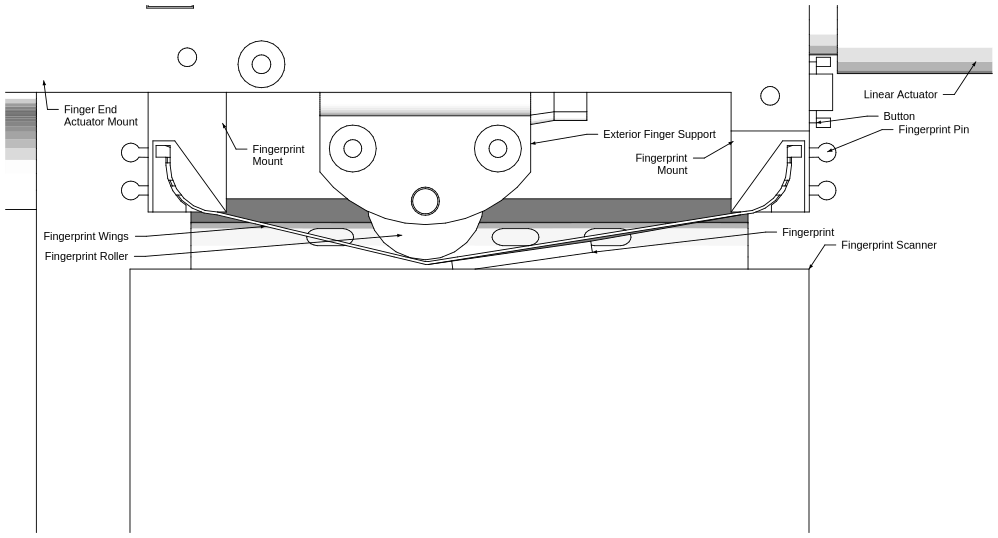
\includegraphics{FingerprintAssembly.pdf}

The linear actuator pulls the roller towards the button. As the roller moves, it compresses the fingerprint against the scanner, causing the scanner the capture a rolled print. Once the moving assembly (consisting of the roller and its support structure) hits the button, the linear actuator stops, and then reverses.


\subsubsection{Electronics Box}
\label{NARFSTR:electronics-box}
The electronics box contains openings for all the connections and buttons on the robot. The following picture shows all the main features:

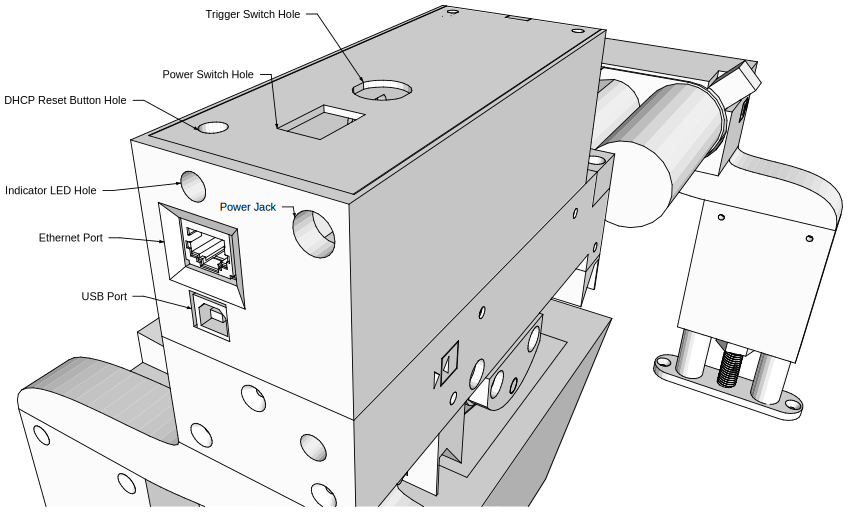
\includegraphics{ElectronicsHousingFront.pdf}

There are also four more openings on the back. These are to allow the linear actuator and the button in the fingerprint assembly to connect to the electronics in the box. The following image shows these connections:

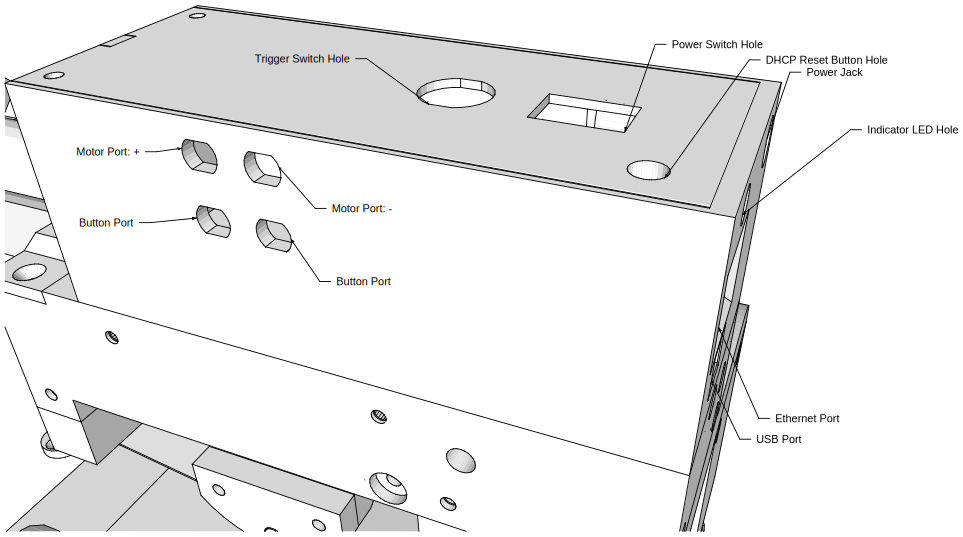
\includegraphics{ElectronicsHousingBack.pdf}


\section{Construction}
\label{NARFSTR:construction}

\subsection{Parts}
\label{NARFSTR:parts}

\subsubsection{3D Printed Parts}
\label{NARFSTR:d-printed-parts}
Almost all of the parts for the robot are 3D printed. The STL files for the parts are located in \code{Final STL Files/NARFSTR}. All of the 3D printed parts were printed in PLA except for the fingerprints. (For more information abou the fingerprints, see {\hyperref[NARFSTR:fingerprintsection]{\emph{\DUspan{}{Fingerprints}}}}.) The PLA parts were printed with a layer height of 0.2 mm using MakerBot's ``Standard'' profile. We used a MakerBot Replicator 2 and a  5$^{\text{th}}$ Generation Replicator. The following table lists each part's name and quantity.


\begin{threeparttable}
\capstart\caption{3D Printed Parts}
\label{NARFSTR:id3}
\begin{tabulary}{\linewidth}{|L|L|}
\hline
\textsf{\relax 
Part Name
} & \textsf{\relax 
Quantity
}\\
\hline
Actuator Mount - Finger End
 & 
1
\\
\hline
Actuator Mount - Motor End
 & 
1
\\
\hline
Actuator Pin - Finger End
 & 
1
\\
\hline
Actuator Pin - Motor End
 & 
1
\\
\hline
Actuator Strap
 & 
1
\\
\hline
Bolt Head
 & 
4
\\
\hline
Button Pusher
 & 
1
\\
\hline
Button Strap
 & 
1
\\
\hline
Electronics Box
 & 
1
\\
\hline
Electronics Box Front Tab
 & 
1
\\
\hline
Electronics Box Side Lid
 & 
1
\\
\hline
Electronics Box Top Lid
 & 
1
\\
\hline
Fingerprint
 & 
1
\\
\hline
Fingerprint Base
 & 
1
\\
\hline
Fingerprint Bracing
 & 
2
\\
\hline
Fingerprint Clip
 & 
2
\\
\hline
Fingerprint Mount - Finger End
 & 
1
\\
\hline
Fingerprint Mount - Motor End
 & 
1
\\
\hline
Fingerprint Roller A
 & 
1
\\
\hline
Fingerprint Roller B
 & 
1
\\
\hline
Leg Connector - Finger End
 & 
1
\\
\hline
Leg Connector - Motor End
 & 
1
\\
\hline
Leg Lower
 & 
4
\\
\hline
Leg Upper
 & 
4
\\
\hline
Lock Nut
 & 
4
\\
\hline
Power Jack Holder
 & 
1
\\
\hline\end{tabulary}

\end{threeparttable}



\subsubsection{Electronic Parts}
\label{NARFSTR:electronic-parts}
The following table lists all the electronic parts. Parts that are marked with * are close to the parts I used, but may not be exact. This is because the parts I used came from kits or other sources, and I was unable to determine their exact information. For the male and female banana plugs, 3 different colors are recommended: 1 red, 1 black, 2 blue.


\begin{threeparttable}
\capstart\caption{Electronic Parts}
\label{NARFSTR:id4}
\begin{tabulary}{\linewidth}{|L|L|L|L|}
\hline
\textsf{\relax 
Part Name
} & \textsf{\relax 
Manufacturer
} & \textsf{\relax 
Number
} & \textsf{\relax 
Quantity
}\\
\hline
10 k\(\Omega\) resistor
 &  &  & 
3
\\
\hline
12 mm push button*
 & 
Sparkfun
 & 
COM-09190
 & 
2
\\
\hline
12V 5A switching power supply
 & 
Adafruit
 & 
352
 & 
1
\\
\hline
20 gauge stranded wire
 &  &  & 
1
\\
\hline
470\(\Omega\) resistor
 &  &  & 
3
\\
\hline
5 cm x 7 cm double sided perfboard
 & 
Amico
 & 
s14011600am1317
 & 
1
\\
\hline
Arduino Ethernet shield
 & 
Arduino
 & 
A000056
 & 
1
\\
\hline
Arduino Uno R3
 & 
Arduino
 & 
A000066
 & 
1
\\
\hline
Common cathode RGB LED*
 & 
Sparkfun
 & 
COM-00105
 & 
1
\\
\hline
Female tab connector
 & 
TE Connectivity / AMP
 & 
3-350820-2
 & 
3
\\
\hline
LED Cap*
 & 
Keystone
 & 
8665
 & 
1
\\
\hline
Linear actuator - 5'' Stroke
 & 
Firgelli Automations
 & 
FA-TR-35-12-5''
 & 
1
\\
\hline
Male tab connector
 & 
TE Connectivity / AMP
 & 
3-520107-2
 & 
3
\\
\hline
Power pigtail female
 & 
Monoprice
 & 
6881
 & 
1
\\
\hline
Solderless banana plug female
 & 
Johnson
 & 
108-0910-001
 & 
4
\\
\hline
Solderless banana plug male
 & 
Johnson
 & 
108-0310-001
 & 
4
\\
\hline
Solid core mounting wire kit
 & 
Velleman Components
 & 
K/MOWM
 & 
1
\\
\hline
SPST 9 amp on off illuminated green
 & 
Jameco Valuepro
 & 
R13-66B-G-02
 & 
1
\\
\hline
Switch push button SPST off momentary (on) red amp LED illuminated
 & 
Jameco Valuepro
 & 
R13-508AL-05-BRR-L3
 & 
1
\\
\hline
UBEC DC/DC step-down (buck) converter - 5V @ 3A output
 & 
Adafruit
 & 
1385
 & 
1
\\
\hline
VNH5019 motor driver carrier
 & 
Pololu
 & 
1415
 & 
1
\\
\hline\end{tabulary}

\end{threeparttable}



\subsubsection{Screws and Miscellaneous Parts}
\label{NARFSTR:screws-and-miscellaneous-parts}
I did not order these parts, and so have limited information about them.


\begin{threeparttable}
\capstart\caption{Screws and Miscellaneous Parts}
\label{NARFSTR:id5}
\begin{tabulary}{\linewidth}{|L|L|L|}
\hline
\textsf{\relax 
Part name
} & \textsf{\relax 
Color
} & \textsf{\relax 
Quantity
}\\
\hline
19 mm diameter rubber feet
 & 
Black
 & 
8
\\
\hline
\#4 US wood screw, 15.7 mm
 & 
Gold
 & 
17
\\
\hline
\#4 US wood screw, 8.5 mm
 & 
Black
 & 
19
\\
\hline
\#8 US machine screw,  12 mm
 & 
Silver
 & 
4
\\
\hline
Epoxy
 &  & \\
\hline
Super glue
 &  & \\
\hline\end{tabulary}

\end{threeparttable}


Here is a picture of the screws:

\includegraphics{screws.jpg}

From now on, I will refer to the screws by their color.


\subsection{Legs and Actuator Mount Assembly}
\label{NARFSTR:legs-and-actuator-mount-assembly}

\subsubsection{Legs}
\label{NARFSTR:legs}
There are two leg assemblies: one on the side of the actuator with the motor, and one on the other side. Both are assembled the same way, but they use different leg adapters. To assemble a leg assembly, first screw a lock nut onto the threaded bolt in the center of the lower adjustable foot. Repeat for the other leg. Then, put an upper adjustable foot piece on top of each lower adjustable foot piece. Push down until the lock nut clicks, locking the lower part to the upper part. Then, insert a bolt head into the square hole on top of each upper adjustable foot. Screw the square head into the bolt using one of the black screws. Finally, connect each foot assembly to the lower part of a leg adapter. Secure the connection by screwing golden screws into the holes on the upper adjustable foot. Repeat this process with the other leg adapter to make the other leg assembly.

\includegraphics{LegAssembly.pdf}


\subsubsection{Actuator Mounts}
\label{NARFSTR:actuator-mounts}
There are two actuator mounts: one for the side of the actuator with the motor, and one for the other side.


\paragraph{Motor End Actuator Mount}
\label{NARFSTR:motor-end-actuator-mount}
Slide the actuator into the mount. Insert the motor end actuator key into the hole in the actuator mount. Make sure the arrows point towards each other. Secure the key with a golden screw.

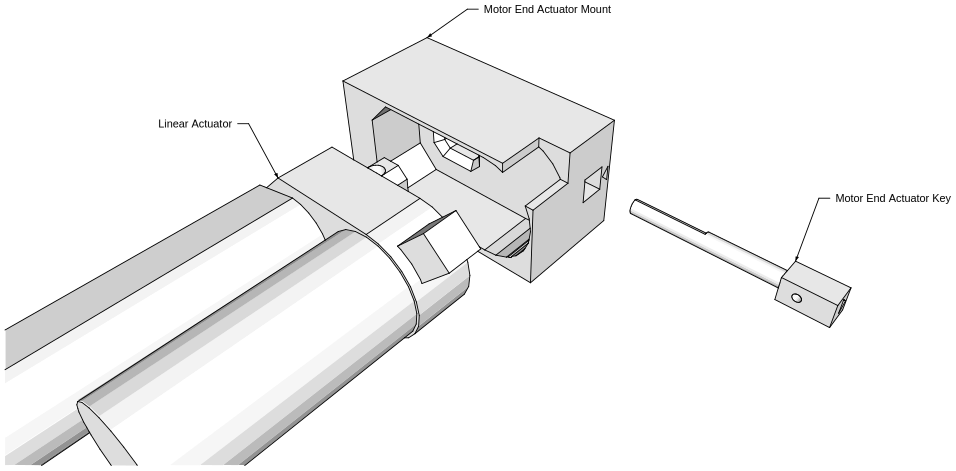
\includegraphics{MotorEndActuatorMount.pdf}


\paragraph{Finger End Actuator Mount}
\label{NARFSTR:finger-end-actuator-mount}
Slide the actuator into the mount. Insert the finger end actuator key into the hole in the actuator mount. Make sure the arrows point towards each other. Attach the top actuator strap to the actuator using two golden screws.

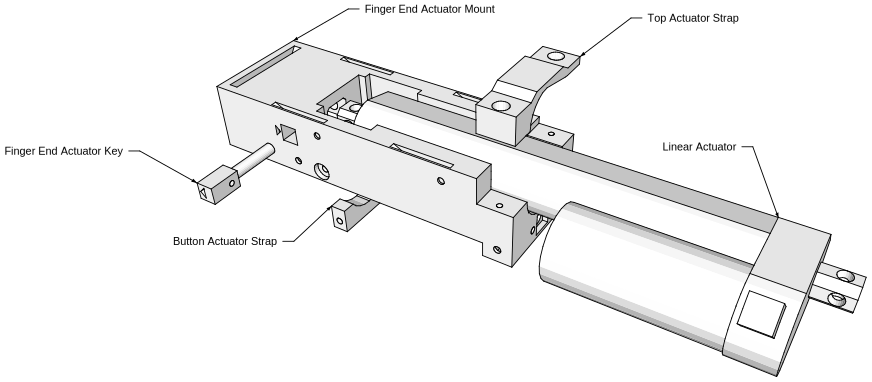
\includegraphics{FingerEndActuatorMount.pdf}

Insert the bottom actuator strap as shown in the diagram below. Secure it with two black screws. Finally, screw a golden screw into the hole labeled ``Screw Hole for Actuator Key'' on the diagram below. This secures the key.

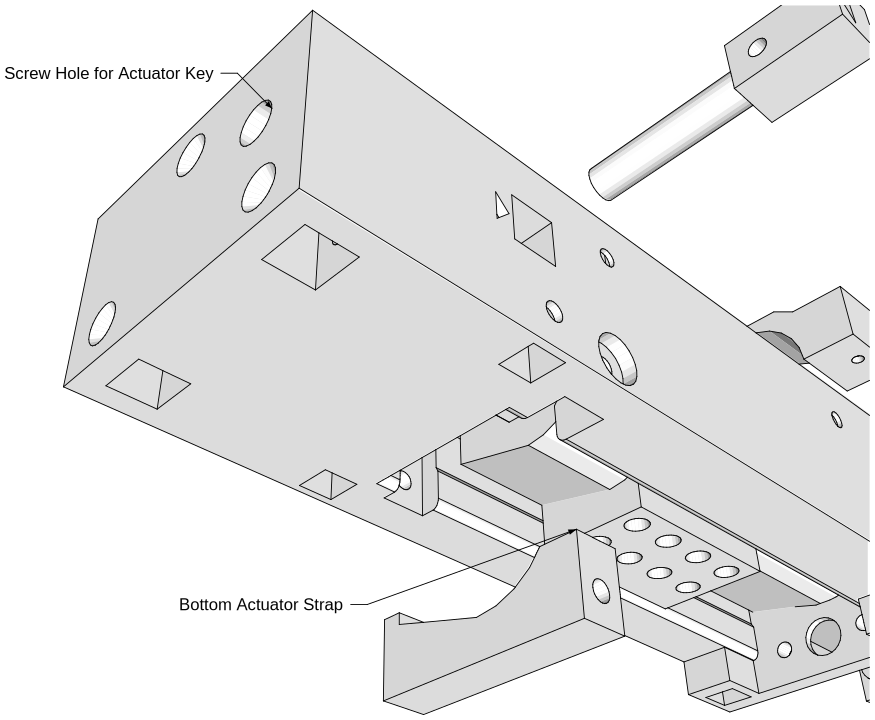
\includegraphics{FingerEndActuatorMountBottom.pdf}

Put a 12 mm push button into the button hole on the actuator mount. Secure the button using the button strap and two black screws.

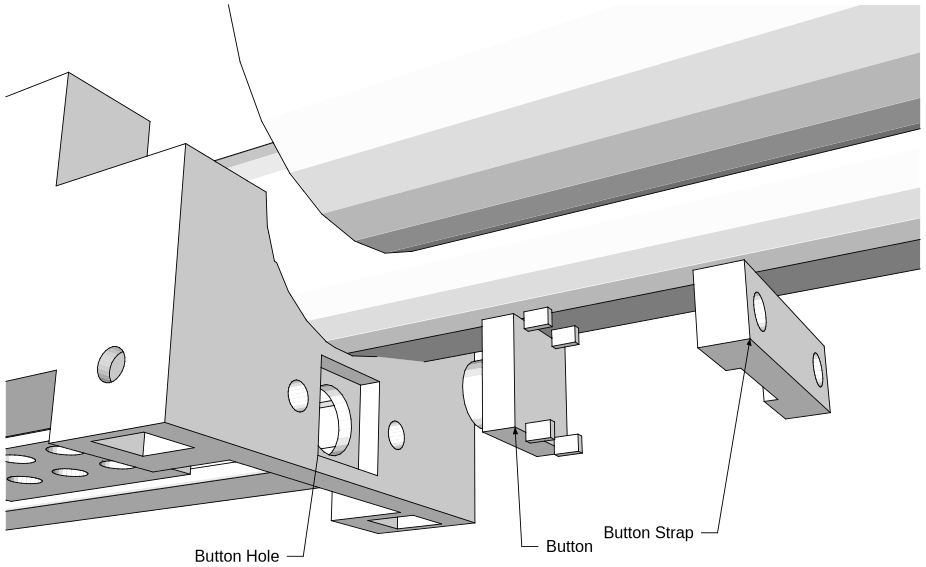
\includegraphics{ButtonInstallation.pdf}

Insert the finger end fingerprint mount and the motor end fingerprint mount into the bottom of the actuator mount. Secure each one with two black screws. Then, insert a fingerprint clip into each of the fingerprint mounts.

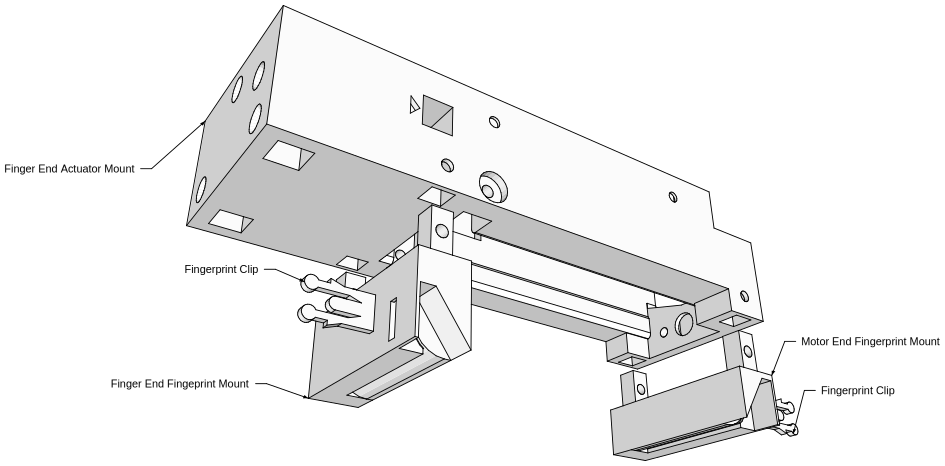
\includegraphics{FingerprintMountInstallation.pdf}


\subsubsection{Connecting the Legs and Actuator Mounts}
\label{NARFSTR:connecting-the-legs-and-actuator-mounts}
Insert the leg assemblies into the bottom of the actuator assembly. Secure each leg assembly with two golden screws.

\includegraphics{LegAttachment.pdf}


\subsubsection{Rubber Feet}
\label{NARFSTR:rubber-feet}
Insert two rubber feet into the bottom of each foot.


\subsection{Fingerprint Assembly}
\label{NARFSTR:id1}
Glue fingerprint roller A into fingerprint roller B using super glue. Let dry. Connect fingerprint roller to moving base with the exterior finger supports. Secure each support with two black screws. Insert the button pusher into the moving base.

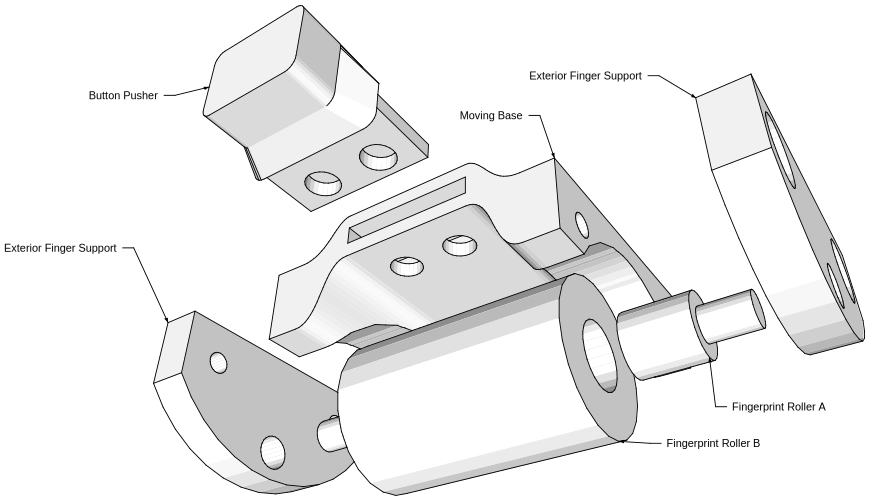
\includegraphics{FingerprintAssemblyConstruction.pdf}

Attach the fingerprint assembly to the actuator by first aligning the four holes on the moving base with the holes on the actuator, ensuring that the button pusher faces the button. Then, screw a silver screw into each of the four holes on the moving base.

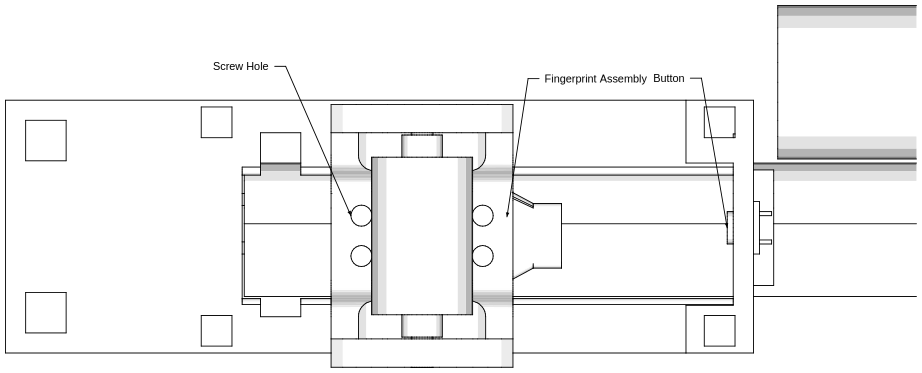
\includegraphics{FingerprintAssemblyInstallation.pdf}


\subsection{Electronics Box Assembly}
\label{NARFSTR:electronics-box-assembly}
\textbf{Note:} assemble the electronics before assembling the box.

Slide Arduino Uno (with Arduino Ethernet Shield) into the box. Screw female banana plugs into holes of electronics housing. If using colors, put a red jack and a black jack into the top row, and put two blue jacks in the bottom row. Then, super glue the LED cap into the LED hole.

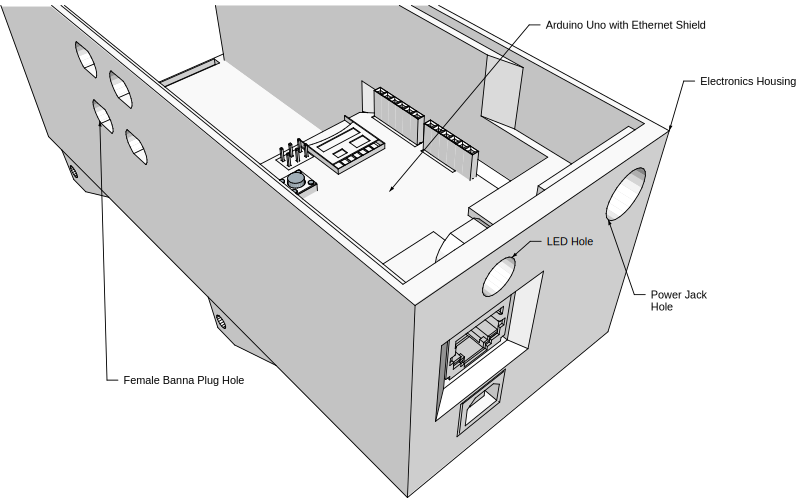
\includegraphics{ArduinoInstallation.pdf}

Super glue the front tab onto the bottom of the electronics box.

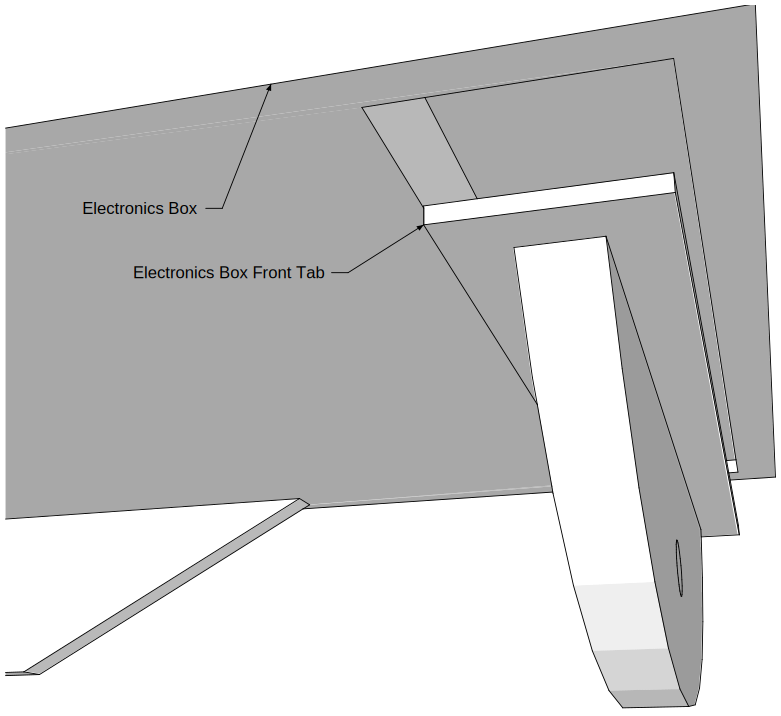
\includegraphics{ElectronicsBoxFrontTabInstallation.pdf}

Assemble the top lid by inserting the power switch and the trigger switch into their holes. The power switch is the green rocker switch, and the trigger switch is the red push button. Using epoxy, glue a 12 mm button into the DHCP reset button hole. The square base of the button should be glued onto the plastic square on the bottom of the top lid.

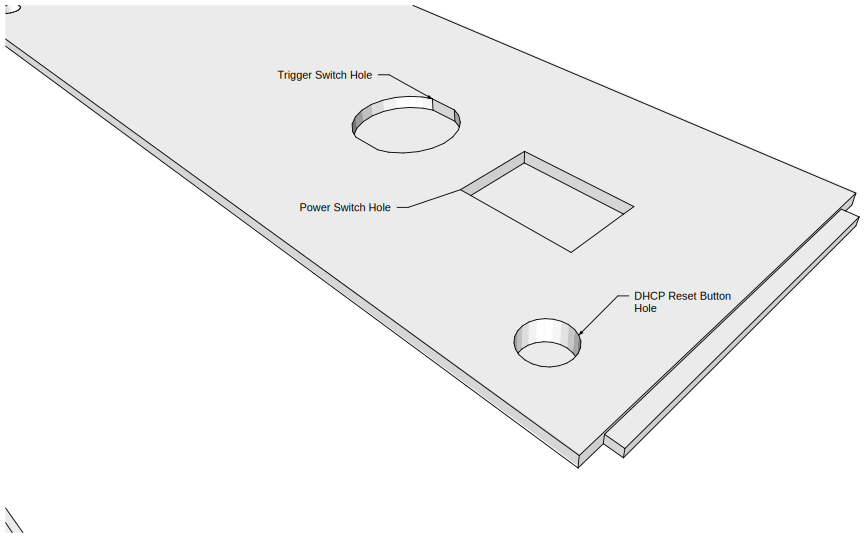
\includegraphics{TopLidButtonInstallation.pdf}

Assemble the power jack by inserting a female power pigtail into the power jack holder. This may require some force. Screw power jack holder into electronics box using a black screw.

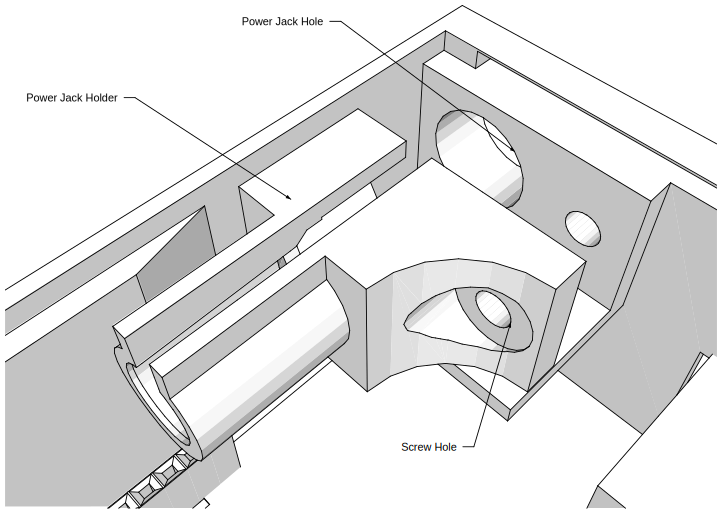
\includegraphics{PowerJackInstallation.pdf}

Put all other electronics into the box in the empty area behind the Arduino and put LED into LED cap. Ensure that everything is properly connected. Then, put top on box and secure with two black screws. Put back side on box and secure with one black screw. Finally, connect all cables.


\section{Electronics}
\label{NARFSTR:electronics}

\subsection{Design}
\label{NARFSTR:id2}
The robot is controlled by an Arduino Uno microcontroller. On top of the Arduino, there is an Arduino Ethernet Shield, which, through its single Ethernet port, allows the robot to connect to a network. The following components are connected to the Arduino through the header pins on the shield:
\begin{enumerate}
\item {} 
RGB LED: serves as an indicator light.

\item {} 
Trigger switch: a red pushbutton, causes the robot to move its finger back and forth when pressed.

\item {} 
Limit switch: a 12 mm push button which detects when the fingerprint has finished rolling.

\item {} 
DHCP reset button: a 12 mm push button, causes the robot to request a DHCP lease.

\item {} 
Pololu VNH5019 motor driver chip: used to drive the linear actuator.

\end{enumerate}

The robot has a single 2.1 mm DC barrel jack for power and requires 12 V DC at around 3A (estimated; based on peak motor current draw). The 12 V lines are attached directly to the motor control board, and the Arduino is powered by the output of a 5V Universal Battery Elimination Circuit (UBEC). The UBEC can produces a regulated 5 V output at a current of up to 3A. This works far better than the Arduino's built-in regulator, which, though it can handle 12 volts, gets very hot when doing so and has trouble providing the necessary current for both the Arduino and the Ethernet Shield. The robot also has a power switch, which is connected to the 12 V input line.

Here is a schematic:

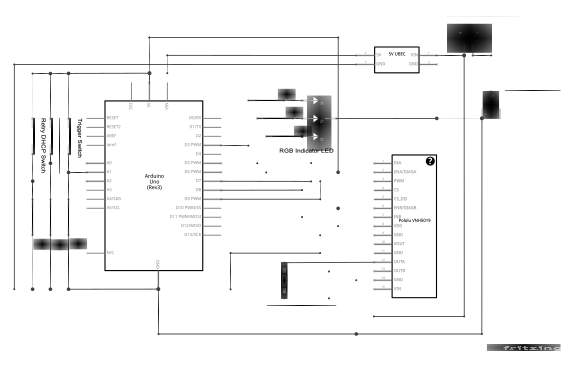
\includegraphics{NARFSTRCircuit_schem.pdf}

There is no Ethernet Shield in the schematic, but it would be placed on top of the Arduino.


\subsection{Assembly}
\label{NARFSTR:assembly}
First, put the Arduino Ethernet Shield onto the Arduino. Then, on the 5 cm x 7 cm perfboard, assemble the circuit using the schematic above. For the motor and limit switch, which are mounted outside of the box, connect their leads to the female banana plugs, which will go into holes on the side of the electronics box. On the ends of the leads for the motor and button (which will be outside the box), attach the male banana plugs. Use the two blue plugs for the button's leads, the red one for the motor's red wire, and the black one for the motor's black wire. For the LED and other buttons, make sure they are connected with long wires so they can reach from the circuit board to their designated location in the box. Also, do not directly connect any components that will be mounted in the box directly to the circuit board. You will not be able to put the components into their holes. Instead, use the tab connectors to attach the component to the rest of the circuit. Finally, on all the 12 V lines (which, because they are connected to the motor, would have high currents), use the 20 gauge wire.


\section{Fingerprints}
\label{NARFSTR:fingerprintsection}\label{NARFSTR:fingerprints}
The fingerprints used on the robot are 3D printed. The first step in making a fingerprint is to generate a PNG image of the fingerprint. To do this, I used \href{http://biolab.csr.unibo.it/research.asp?organize=Activities\&select=\&selObj=12\&pathSubj=111\%7C\%7C12\&}{SFinGe} (http://biolab.csr.unibo.it/research.asp?organize=Activities\&select=\&selObj=12\&pathSubj=111\%7C\%7C12\&) (\textbf{S}ynthetic \textbf{Fin}gerprint \textbf{Ge}nerator) from the Biometric System Laboratory at the University of Bologna . With the program, I configured various parameters of the fingerprint, and once the ridges were generated, clicked the ``View original'' button after every step to remove all the distortion and scratches. Once the fingerprint was generated, I saved it to a bmp file and then converted it to a png.

To turn the PNG into a 3D-printable file, I wrote an OpenSCAD script, located at \code{Fingerprints/NARFSTRRolledFingerprints/roll.scad}. This script can take any black and white PNG image and produce a STL file that, when 3D printed, will fit perfectly into the robot. To use the script, configure the variables at the top of the file:

\begin{Verbatim}[commandchars=\\\{\}]
imageResolution = 19.7; //dots per mm
imageX = 416; //px
imageY = 560; //px
file = \PYGZdq{}FGen1.png\PYGZdq{};
fingerprintX = 30; //mm
fingerprintY = 30; //mm
fingerprintScale = 1.4;
\end{Verbatim}

Once these variables are configured, hit ``Preview'' in OpenSCAD to make sure everything looks good, and then hit ``Render''. This may take about an hour. Once the rendering is complete, export the file as an STL.

This script will generate a very complex 3D file which contains the fingerprint, mounted on a spongy area, which is mounted on tabs that connect to the robot. Here is a cross-sectional view of the finished product:


\includegraphics{LabeledFingerprint.pdf}

The two tabs at either end allow the fingerprint to be secured to the robot. The fingerprint is on top of the raised area in the middle. The holes in the raised area allow the fingerprint to compress, which results in a better scan. Here is a close up view of the holes:

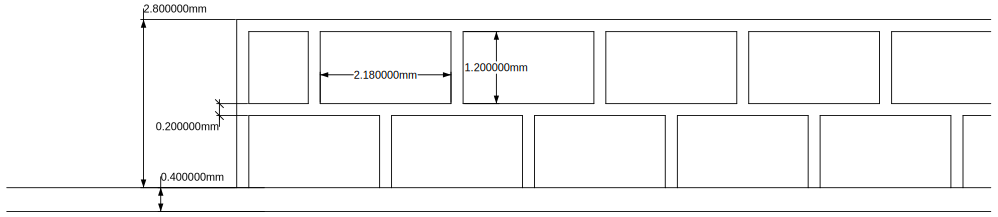
\includegraphics{LabeledFingerprintZoomed.pdf}

To 3D print the STL file, use MakerBot Flexible Filament. Be sure to set the printing profile to the custom profile located at \code{Fingerprints/ NARFSTR Rolled Fingerprints/fingerprintprofile.txt}. The custom profile, which is based off of the MakerBot flexible filament profile, uses 1 shell and an extruder temperature of 140 °C.


\chapter{NAFSTR}
\label{NAFSTR::doc}\label{NAFSTR:nafstr}
\textbf{Note:} The documentation below is sparse and needs to be improved. Have fun!


\section{Design}
\label{NAFSTR:design}
Here is an image showing the main parts of the robot:

\includegraphics{Scene1N.pdf}

Here is an exploded view of the robot, which is helpful for assembly:

\includegraphics{Scene5N.pdf}

Here is an image showing how the finger attaches to the servo and how the fingerprint attaches to the finger:

\includegraphics{Scene2N.pdf}

Here is an image showing how the robot rests on the fingerprint scanner:

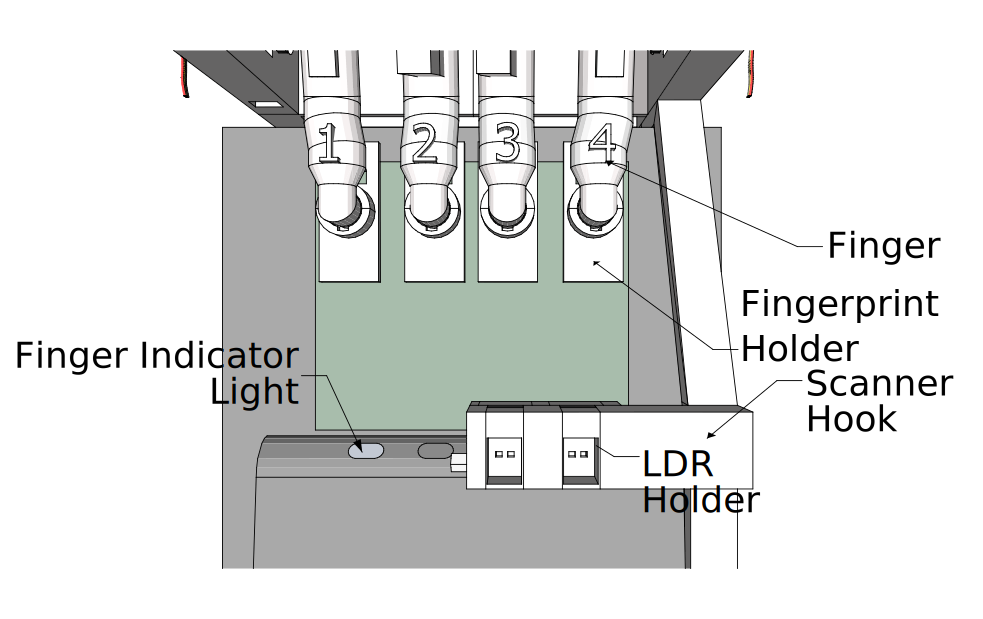
\includegraphics{Scene3N.pdf}

Here is a final image showing how the electronics housing is assembled:

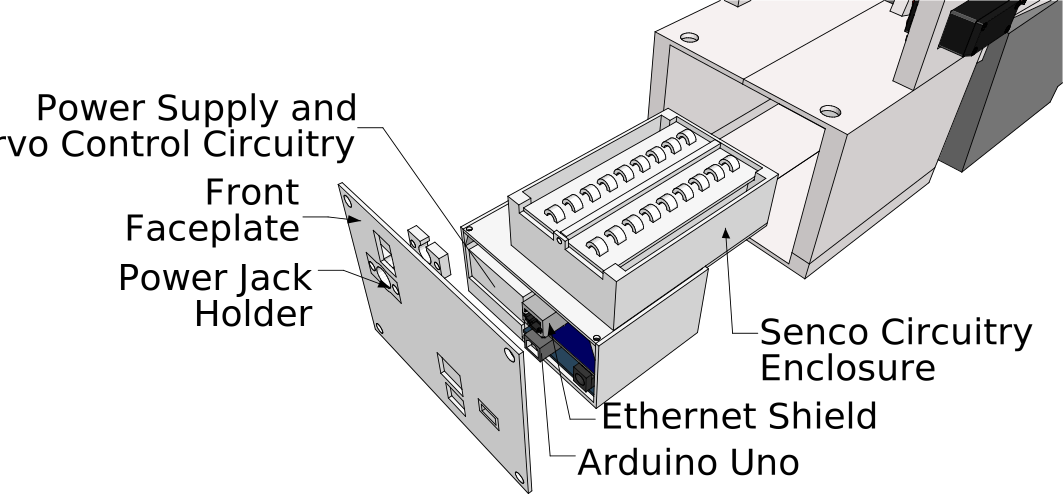
\includegraphics{Scene4N.pdf}


\section{Construction}
\label{NAFSTR:construction}
To construct the robot, first print appropriate quantities of the parts in \code{Final STL Files/NAFSTR}. Then, attach all the parts together and insert all the electronics. Here is a parts list of all the required parts that are not 3D printed:


\begin{threeparttable}
\capstart\caption{Parts of NAFSTR}
\label{NAFSTR:id1}
\begin{tabulary}{\linewidth}{|L|L|L|L|L|}
\hline
\textsf{\relax 
Part Name
} & \textsf{\relax 
URL
} & \textsf{\relax 
Quantity
} & \textsf{\relax 
Price
} & \textsf{\relax 
Total Price
}\\
\hline
Photoresistor GL5537 5537
 & 
\href{http://www.amazon.com/gp/product/B008QVE9BG/ref=ox\_sc\_act\_title\_1?ie=UTF8\&psc=1\&smid=A39BKDU4I2L317}{http://www.amazon.com/gp/product/B008QVE9BG/ref=ox\_sc\_act\_title\_1?ie=UTF8\&psc=1\&smid=A39BKDU4I2L317}
 & 
4
 & 
0.2475
 & 
0.99
\\
\hline
1/2'' Circular Force Sensing Resistor
 & 
\href{http://www.jameco.com/webapp/wcs/stores/servlet/Product\_10001\_10001\_2128260\_-1}{http://www.jameco.com/webapp/wcs/stores/servlet/Product\_10001\_10001\_2128260\_-1}
 & 
4
 & 
7.95
 & 
31.8
\\
\hline
Hitech HS645MG Servo Motor
 & 
\href{http://www.amazon.com/Hitec-32645S-HS-645MG-Torque-Metal/dp/B003T6RSVQ}{http://www.amazon.com/Hitec-32645S-HS-645MG-Torque-Metal/dp/B003T6RSVQ}
 & 
4
 & 
49.99
 & 
199.96
\\
\hline
Arduino Uno
 & 
\href{https://www.sparkfun.com/products/11021}{https://www.sparkfun.com/products/11021}
 & 
1
 & 
24.95
 & 
24.95
\\
\hline
Arduino Ethernet Shield
 & 
\href{https://www.sparkfun.com/products/9026}{https://www.sparkfun.com/products/9026}
 & 
1
 & 
45.95
 & 
45.95
\\
\hline
Rocker Switch On Off Single Pole Single Throw Quick Connect Rocker 10 Amp 250 Volt AC Straight
 & 
\href{http://www.jameco.com/webapp/wcs/stores/servlet/Product\_10001\_10001\_316128\_-1}{http://www.jameco.com/webapp/wcs/stores/servlet/Product\_10001\_10001\_316128\_-1}
 & 
1
 & 
1.65
 & 
1.65
\\
\hline
DC Power Pigtail Female Plug
 & 
\href{http://www.monoprice.com/Product?seq=1\&format=2\&p\_id=6881\&CAWELAID=1329453851\&CAGPSPN=pla\&gclid=CjwKEAjw9eyeBRCqxc\_b-LD8kTESJADsBMxSlZYFRPGB2LwI09oGs0PsjcrUS6Nd1nQFYJR-kuWp-BoCAAjw\_wcB}{http://www.monoprice.com/Product?seq=1\&format=2\&p\_id=6881\&CAWELAID=1329453851\&CAGPSPN=pla\&gclid=CjwKEAjw9eyeBRCqxc\_b-LD8kTESJADsBMxSlZYFRPGB2LwI09oGs0PsjcrUS6Nd1nQFYJR-kuWp-BoCAAjw\_wcB}
 & 
1
 & 
0.48
 & 
0.48
\\
\hline
5V 3A UBEC
 & 
\href{http://www.adafruit.com/products/1385}{http://www.adafruit.com/products/1385}
 & 
5
 & 
9.95
 & 
49.75
\\
\hline
Multiplexer CD74HC4067E
 & 
\href{http://www.digikey.com/product-detail/en/CD74HC4067E/296-33087-5-ND/1507234}{http://www.digikey.com/product-detail/en/CD74HC4067E/296-33087-5-ND/1507234}
 & 
1
 & 
2.33
 & 
2.33
\\
\hline
1 k\(\Omega\) Resistor
 & 
\href{http://www.jameco.com/webapp/wcs/stores/servlet/Product\_10001\_10001\_690865\_-1}{http://www.jameco.com/webapp/wcs/stores/servlet/Product\_10001\_10001\_690865\_-1}
 & 
15
 & 
0.099
 & 
1.485
\\
\hline
Jumper Wires
 &  & 
100
 &  & 
0
\\
\hline
Solid Core Wire (22 Gauge)
 &  &  &  & 
0
\\
\hline
Mini Breadboard
 & 
\href{https://www.sparkfun.com/products/12043}{https://www.sparkfun.com/products/12043}
 & 
2
 & 
3.95
 & 
7.9
\\
\hline
Half Breadboard
 & 
\href{https://www.sparkfun.com/products/12002}{https://www.sparkfun.com/products/12002}
 & 
1
 & 
4.95
 & 
4.95
\\
\hline
10 \(\mu\)F Capacitor
 & 
\href{https://www.sparkfun.com/products/523}{https://www.sparkfun.com/products/523}
 & 
1
 & 
0.45
 & 
0.45
\\
\hline
10x Single Row Male and Female 40 Pin Header Strip 2.54mm / Square Pin Type, Single Row Pin Header Strips, Great Components for PCB
 & 
\href{http://www.amazon.com/Single-Female-Header-2-54mm-Components/dp/B008QUVM4E}{http://www.amazon.com/Single-Female-Header-2-54mm-Components/dp/B008QUVM4E}
 & 
1
 & 
5.24
 & 
5.24
\\
\hline
12V 5A Switching Power Supply
 & 
\href{https://www.adafruit.com/products/352}{https://www.adafruit.com/products/352}
 & 
1
 & 
24.95
 & 
24.95
\\
\hline
Total:
 &  &  &  & 
402.835
\\
\hline\end{tabulary}

\end{threeparttable}



\section{Electronics}
\label{NAFSTR:electronics}
To assemble to electronics, look at the Fritzing file located at: \code{Circuit/NAFSTRCircuit.fzz}.


\chapter{Program Development}
\label{ProgramDevelopment:program-development}\label{ProgramDevelopment::doc}
There are two programs associated with each robot: (1) a Java program that runs on a computer and controls the robot and (2) a C++ program that runs on the robot. The Java program works with both a Graphical User Interface (GUI) and the command line. With the GUI, the user specifies the actions for the robot to execute, and then connects to the robot and executes the actions. With the command line, the user can supply a text file of commands for the robot to execute, and the program will send the commands to the robot. The C++ program on the robot receives all the commands and executes them. It also responds to any button presses.


\section{Java Robot Control Program}
\label{ProgramDevelopment:java-robot-control-program}
The Java program has 3 main parts:
\begin{enumerate}
\item {} 
The back end, which handles all communication with the robot.

\item {} 
The GUI, which provides a simple way to control the robot.

\item {} 
The command line interface, which lets the user send a list of commands to the robot.

\end{enumerate}

This guide will explain each of the three parts.


\subsection{Back End}
\label{ProgramDevelopment:back-end}
The back end consists of the robot package, which contains four main classes:
\begin{enumerate}
\item {} 
\code{Robot}

\item {} 
\code{RobotCom}

\item {} 
\code{RobotInfo}

\item {} 
\code{Command}

\end{enumerate}

\code{Robot} is an abstract class, and it represents any type of robot, either a NAFSTR or a NARFSTR. It currently has one subclass, \code{NARFSTR}. The current version of the program does not support the NAFSTR robot; to control a NAFSTR, the older version must be used. \code{NARFSTR} has one constructor, which takes a \code{RobotCom} object. A \code{RobotCom} is a channel for communicating with the robot, and has methods for reading and writing data. \code{RobotCom} has two subclasses: \code{SerialRobotCom}, which represents a connection to a robot over a serial port (USB), and \code{NetworkRobotCom}, which represents a connection to a robot over a network. In order to make an instance of either class, a \code{RobotInfo} object is required. A \code{RobotInfo} object describes the type of robot, the location of the robot (an IP address and a serial port), and the robot's MAC address, which is used as an ID.

In order to easily find robots, the \code{Robot} class provides three static methods:
\begin{enumerate}
\item {} 
\code{findSerialRobots()}: finds all the robots connected over USB by checking every USB port.

\item {} 
\code{findNetworkedRobots()}: finds all the robots connected over the network by sending out a UDP broadcast and listening for responses.

\item {} 
\code{findRobots()}: finds all the robots over both USB and the network.

\end{enumerate}

In order to execute commands on a robot, the \code{Robot} class provides an \code{executeCommand(Command c)} method, and an \code{executeCommands(List\textless{}Command\textgreater{} commands)} method. Both methods send commands to the robot, and wait for execution to finish. A \code{Command} object consists of two components: a String representing the command name, and a list of Objects representing the parameters.

For more documentation, see the Javadoc, in \code{Code/FingerprintRobotControl/doc}.


\subsection{GUI}
\label{ProgramDevelopment:gui}
The code for the GUI is in three packages: \code{view}, \code{view.configurator}, and \code{view.robotpanel}. The program's GUI is an instance of \code{view.RobotController}. The \code{RobotController} class has two main components: a \code{view.robotpanel.RobotConnectionPanel}, which manages the connection with the robot, and a \code{view.robotpanel.CommandEditorPanel}, which allows the user to edit the commands being sent to the robot.


\subsection{Command Line}
\label{ProgramDevelopment:command-line}
The code for the command line interface is in \code{main.FingerprintRobotControl}. When \code{FingerprintRobotControl} is executed with no arguments, it automatically creates an instance of \code{view.RobotController}, creating the GUI. If there are arguments, it attempts to use them. The argument format is: \code{\textless{}robot type\textgreater{} \textless{}file name\textgreater{} \textless{}connection location\textgreater{}}. The robot type should be either NAFSTR of NARFSTR. (NAFSTR is not currently supported, but will be soon.) The file name should be an absolute or relative path to the file of commands which the program is to execute. The file format is a text file with one command per line. Finally, the connection location could be one of four things: ``ethernet'', ``usb'', an IP address, or a serial port. If it is ``ethernet'' or ``usb'', to program will search for robots connected over the specified channel, and pick the first one.


\section{C++ Local Control Program}
\label{ProgramDevelopment:c-local-control-program}

\subsection{Development Environment}
\label{ProgramDevelopment:development-environment}
The program was developed in Eclipse using the the Arduino Eclipse Extensions version 2.4.201506210212 by Jan Baeyens (\href{http://www.baeyens.it/eclipse/}{http://www.baeyens.it/eclipse/}), with the Arduino libraries version 1.6.5. The Robot's program consists of two parts: C++ libraries which are common to both robots (the libraries are currently only used with the NARFSTR, but should be used on the NAFSTR), and a \code{.ino} file which contains the main program for the robot. The \code{FingerprintRobotCom} library is stored in \code{Code/FingerprintRobotLocalControl/lib}. In order to make the Arduino plugin include this library (and other libraries which are stored in the lib folder) in the build path, the ``Private Library Path'' in the Arduino Plugin Preferences must be set to \code{Code/FingerprintRobotLocalControl/lib}.


\subsection{Libraries}
\label{ProgramDevelopment:libraries}
The code needs several libraries in order to compile. First, it needs the \code{FingperintRobotCom} library, which handles communication between the robot and the computer. Second, it needs the \code{EthernetNonBlocking} library, which is a modified version of the standard Arduino Ethernet Library. I modified the standard library to make the DHCP functions non-blocking. This significantly improves responsiveness; with the standard blocking DHCP functions, the robot would freeze for 60 seconds if no Ethernet cable was plugged in. Both programs also need the following standard Arduino libraries:
\begin{enumerate}
\item {} 
\code{EEPROM}

\item {} 
\code{SPI}

\end{enumerate}

Each of the NAFSTR and NARFSTR programs also require some specific libraries:

NAFSTR
\begin{enumerate}
\item {} 
\code{Servo}: standard Arduino library.

\end{enumerate}

NARFSTR
\begin{enumerate}
\item {} 
\code{Arduino-RGB-Tools}: an open-source library for controlling RGB LEDs. It is on github (\href{https://github.com/joushx/Arduino-RGB-Tools}{https://github.com/joushx/Arduino-RGB-Tools}), stored in the git repository as a submodule, and licensed under The MIT License (MIT).

\item {} 
\code{RGBConverter}:  an open-source library for converting between RGB and HSV. It is on github (\href{https://github.com/ratkins/RGBConverter}{https://github.com/ratkins/RGBConverter}), stored in the git repository as a submodule, and its license says that you can do whatever you want with it.

\item {} 
\code{VNH5019Driver}: a library I wrote for controlling the VNH5019 driver chip.

\end{enumerate}


\subsection{NARFSTR}
\label{ProgramDevelopment:narfstr}
The NARFSTR control program is located at \code{Code/FingerprintRobotLocalControl/NARFSTRLocalControl}. Its main file is \code{NARFSTRLocalControl.ino}.


\subsection{NAFSTR}
\label{ProgramDevelopment:nafstr}
The NAFSTR control program is located at \code{Code/FingerprintRobotLocalControl/NAFSTRLocalControl}. Its main file is \code{NAFSTRLocalControl.ino}. The NAFSTR program is old, and so does not use either the \code{FingerprintRobotCom} library or the \code{EthernetNonBlocking} library.


\subsection{Development Information}
\label{ProgramDevelopment:development-information}
The \code{FingerpintRobotCom} library attempts to read a MAC address from the Arduino's EEPROM on startup. If no MAC address is found, it will not work. In order to load a MAC address into EEPROM for the first time, use the \code{MACUploader} program located at \code{Code/FingerprintRobotLocalControl/MACUploader}.


\subsubsection{\texttt{FingerprintRobotCom} Library}
\label{ProgramDevelopment:fingerprintrobotcom-library}
The \code{FingerprintRobotCom} library header file (located at \code{Code/FingerprintRobotLocalControl/lib/FingerprintRobotCom/FingerprintRobotCom.h}) contains comments which explain all the important functions.


\chapter{Using the Robots}
\label{Use:using-the-robots}\label{Use::doc}
The robots are controlled by text commands send to them over either a serial connection, a TCP network connection, or a UDP network connection. These text commands can be sent in many ways. They can be sent through the Java control software, using both the command line interface and the GUI, they can be sent using Telnet or Putty, and they can be sent using serial terminal, such as gtkterm. This guide will explain the command format, and how to send commands using all the different channels.


\section{Communication Protocol}
\label{Use:communication-protocol}

\subsection{Protocol}
\label{Use:protocol}

\subsubsection{General Information}
\label{Use:general-information}\begin{enumerate}
\item {} 
The robot will receive input from a serial stream via USB or over a network connection on port 2424 (the NAFSTR uses port 80 because its software is old) via Ethernet. The format of the requests will be the same in all cases.

\item {} 
When the robot is connected over the network, it is capable of receiving requests over both a UDP connection and a TCP connection. However, if any request is received over a UDP connection, the response message will be sent over a TCP connection.

\item {} 
With the exception of UDP messages as mentioned above, the robot will respond to all messages over the channel the message was received on.

\item {} 
The robot only has a 64 byte serial buffer. Thus, if many commands are sent rapidly over USB, some commands will be lost. However, when connected over Ethernet, the robot has a 16 kibibyte buffer, thus making an overflow less likely.

\end{enumerate}


\subsubsection{Format}
\label{Use:format}\begin{enumerate}
\item {} 
Each command has the format \code{commandName arg\_0 arg\_1 arg\_2...}, where \code{arg\_n} is the n$^{\text{th}}$ argument. If the command has no arguments, then the command is simply the name. Each part of the command is separated from the others with a single space.

\item {} 
Upon receiving and successfully parsing a command, the robot will send a message of the format \code{commandName-received}. If there is a problem parsing a command, the robot will instead send \code{bad-command}.

\item {} 
Upon completion of a command, the robot will send a message of the format \code{commandName-end}.

\item {} 
When sent the string “fingerrobot”, the robot will respond with a string of the format: \code{found:robot type:MAC Address:}. For example, a NARFSTR robot with a MAC address of \code{ba:db:ad:ba:db:ad} would respond with \code{found:NARFSTR:ba:db:ad:ba:db:ad:}.

\end{enumerate}


\subsection{Commands}
\label{Use:commands}

\subsubsection{NARFSTR Commands}
\label{Use:narfstr-commands}\begin{quote}\begin{description}
\item[{Stroke}] \leavevmode\begin{quote}\begin{description}
\item[{Description}] \leavevmode
causes the robot to move the finger through one cycle.

\item[{Format}] \leavevmode
\code{stroke}

\end{description}\end{quote}

\item[{Set}] \leavevmode\begin{quote}\begin{description}
\item[{Description}] \leavevmode
sets the parameters of the robot's following moves.

\item[{Format}] \leavevmode
\code{set forwardSpeed buttonWaitTime reverseSpeed returnWaitTime}

\item[{Parameters}] \leavevmode\begin{quote}\begin{description}
\item[{\code{forwardSpeed}}] \leavevmode
the motor's speed when driving the finger away from the starting position. Between 0 and 255, inclusive.

\item[{\code{buttonWaitTime}}] \leavevmode
the amount of time, in ms, the robot should wait once the finger hits the limit switch.

\item[{\code{reverseSpeed}}] \leavevmode
the motor's speed when driving the finger back to the starting position. Between 0 and 255, inclusive.

\item[{\code{returnWaitTime}}] \leavevmode
the amount of time to wait, in ms, once the finger has returned to its original position.

\end{description}\end{quote}

\end{description}\end{quote}

\item[{Reset}] \leavevmode\begin{quote}\begin{description}
\item[{Description}] \leavevmode
causes the robot the drive the finger towards the starting position.

\item[{Format}] \leavevmode
\code{reset time speed}

\item[{Parameters}] \leavevmode\begin{quote}\begin{description}
\item[{\code{time}}] \leavevmode
the amount of time the finger will be in motion, in ms.

\item[{\code{speed}}] \leavevmode
the motor's speed, between 0 and 255 inclusive.

\end{description}\end{quote}

\end{description}\end{quote}

\end{description}\end{quote}


\subsubsection{NAFSTR Commands}
\label{Use:nafstr-commands}
See \code{DocumentationOld/Arduino - Computer Communication Protocol.docx} or \code{DocumentationOld/Arduino - Computer Communication Protocol.txt} for details.


\subsection{Examples}
\label{Use:examples}
The following are examples of what an exchange with the robot would look like.


\subsubsection{NARFSTR Example}
\label{Use:narfstr-example}
\begin{Verbatim}[commandchars=\\\{\}]
fingerrobot
found:NARFSTR:90:a2:da:0f:95:39:
set 120 2000 120 2000
set\PYGZhy{}received
set\PYGZhy{}end
stroke
stroke\PYGZhy{}received
stroke\PYGZhy{}end
reset 1000 255
reset\PYGZhy{}received
reset\PYGZhy{}end
notacommand
bad\PYGZhy{}command
\end{Verbatim}


\subsubsection{NAFSTR Example}
\label{Use:nafstr-example}
Please put one here!


\section{Control with \texttt{FingerpintRobotControl} Java Program}
\label{Use:control-with-fingerpintrobotcontrol-java-program}
The program can be found in \code{Code/FingerprintRobotControl/FingerprintRobotControl-v1.1.jar} and allows for both GUI and command line operation. The following two sections describe both methods.

\textbf{Note:} the NAFSTR uses an older version of the software, found in \code{Code/FingerprintRobotControl/FingerprintRobotControl-v1.0.jar}. Most, but not all, of the instructions below apply to the older version.


\subsection{GUI Control}
\label{Use:gui-control}
To launch the program in GUI mode, simply run the program. Or, launch the program from the command line with no arguments: \code{java -jar FingerprintRobotControl-v1.1.jar}. Once the program opens, you should see a window like the one below.

\includegraphics{JavaProgramEmpty.PNG}

This is the starting screen. To use the program, first search for robots by clicking the ``Search'' button. After about three seconds, the combo box will be populated with the types, locations, and MAC addresses of all the robots the program found. To connect to a robot, select one from the list and press connect. If the connection was successful, the status field to the left of the combo box should say ``Connected''.

Now, you can begin to write the commands you want the robot to execute. There are two ways to do this: (1) using the graphical configurator, which requires no knowledge of the communication protocol or, (2), using the text configurator, which allows you to simply type the commands you wish to send to the robot. To use the graphical configurator, press the button on the bottom of the screen with the name of the command you wish to add. A command should show up on the screen. Now, type in the specified values. A complete graphical program looks like the one below.

\includegraphics{JavaProgramGraphicalConfigurator.PNG}

To use the text configurator, select the tab labeled ``Text Configurator''. If you have a program currently open if the graphical configurator, it will automatically be converted to text and displayed in the text configurator. This is a good way to learn the text format of the commands. Once you are in the text configurator, simply type commands. A program written with the text configurator is shown below:

\includegraphics{JavaProgramTextConfigurator.PNG}

Once you are done with you program, you can save it by going to ``File'' menu and clicking ``Save''. This will bring up a dialog asking you where you would like to save your file. The saved files are plain text files, with the same content that appears in the text configurator. To open a file, choose ``Open'' from the ``File'' menu. When you open a file, there will be radio buttons on the right side of the open dialog to allow you to choose the type of robot the opened file is for. (Currently, there is only one button for the NARFSTR. Support will be added for the NAFSTR in the future.) The picture below shows the open dialog.

\includegraphics{JavaProgramOpenWindow.PNG}

To execute your programs, hit the ``Execute'' button. This will send the commands to the robot. You can see the progress in the progress bar. If you want to stop execution, hit the ``Stop'' button. This will stop execution after the currently running move is complete. There is no way to stop execution in the middle of a move. If you click the stop button, and the program still says ``Stopping'' under the progress bar even though the robot has stopped, you may need to click the ``Force Stop'' button. This will immediately disconnect the robot.


\subsection{Command Line Control}
\label{Use:command-line-control}
To run the program from the command line, use the following command:

\code{java -jar FingerprintRobotControl-v1.1.jar robotType fileName connectionMode}
\begin{quote}\begin{description}
\item[{Parameters}] \leavevmode\begin{quote}\begin{description}
\item[{\code{robotType}}] \leavevmode
the type of robot to control, either NAFSTR or NARFSTR. (Currently only NARFSTR is supported.)

\item[{\code{fileName}}] \leavevmode
an absolute or relative path to a file containing the commands to execute, 1 command per line.

\item[{\code{connectionMode}}] \leavevmode\begin{quote}\begin{description}
\item[{\code{ethernet}}] \leavevmode
searches for robots on the network and connects to the first one found.

\item[{\code{usb}}] \leavevmode
searches for robots connected over USB and connects to the first one found.

\item[{IP address}] \leavevmode
the IP address of the robot to connect to.

\item[{Serial port}] \leavevmode
the name of a serial port the robot is plugged into.

\end{description}\end{quote}

\end{description}\end{quote}

\end{description}\end{quote}


\section{Control Using Telnet, Putty, and other Terminals}
\label{Use:control-using-telnet-putty-and-other-terminals}
The robot can easily be controlled using any terminal. With telnet, simply type \code{telnet ipAddress 2424}, where \code{ipAddress} is the IP address of your robot. With Putty, enter the IP address of your robot and the port 2424. Then, select telnet for the protocol and hit connect. For gtkterm, launch the terminal and select the right serial port. Once you have connected your terminal, just type commands, 1 per line, and the robot should execute them.



\renewcommand{\indexname}{Index}
\printindex
\end{document}
